\section{Durchführung}
\label{sec:durch}
Um eine Zeeman Aufspaltung zu beobachten wird eine Cadmium-Spektrallampe in ein äußeres Magnetfeld gebracht, welches durch 2 Elektromagneten erzeugt wird. Hinter der Spektrallampe befinden 
sich Linsen und andere optische Aufbauten, mithilfe derer das Licht fokussiert, sowie gerichtet werden kann. Am Ende des Aufbaus ist eine Lummer-Gehrcke-Platte, in welche eine 
Digital Kamera gerichtet ist. Zusätzlich befindet sich im Aufbau noch ein Polarisationsfilter, ein Platte mit einem Spalt, sowie ein Geradansichtprisma. Der Aufbau ist schematisch in \autoref{fig:aufbau} dargestellt.

\vspace{-5pt}
\begin{figure}[H]
    \centering
    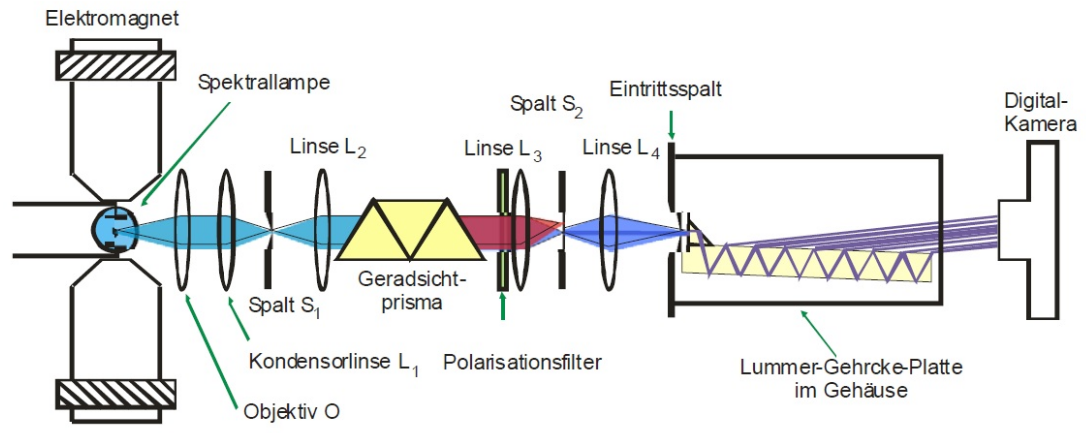
\includegraphics[scale=0.3]{aufbau.png}
    \caption{schematischer Versuchsaufbau \cite{V27}.}
    \label{fig:aufbau}
\end{figure}

\noindent
In $\vec{B}$-Richtung bzw. longitudinaler Richtung ist das linear $\pi$-polarisierte Spektrallicht
nicht zu erkennen, jedoch kann die Händigkeit des zirkular $\sigma^{+}$/$\sigma^{-}$-polarisierten Lichtes
unterschieden werden. In transversaler Richtung, senkrecht zu $\vec{B}$ ist das $\pi$-polarisierte Licht
zu sehen, allerdings erscheint zirkular polarisiertes Licht ebenfalls linear polarisiert.
Dieser Sachverhalt ist auch in Abbildung \ref{fig:pol} dargestellt. Ohne angelegtes Magnetfeld
wird nur $\pi$-polarisiertes Licht beobachtet. 

\noindent
Im Versuchsaufbau wird nur der Lichtstrahl in senkrechte Richtung zum Magnetfeld analysiert, sodass mithilfe des Polarisationsfilters je nach Stellung entweder das linear oder
aber das zirkular polarisierte Licht rausgefiltert wird.

\vspace{-5pt}
\begin{figure}[H]
    \centering
    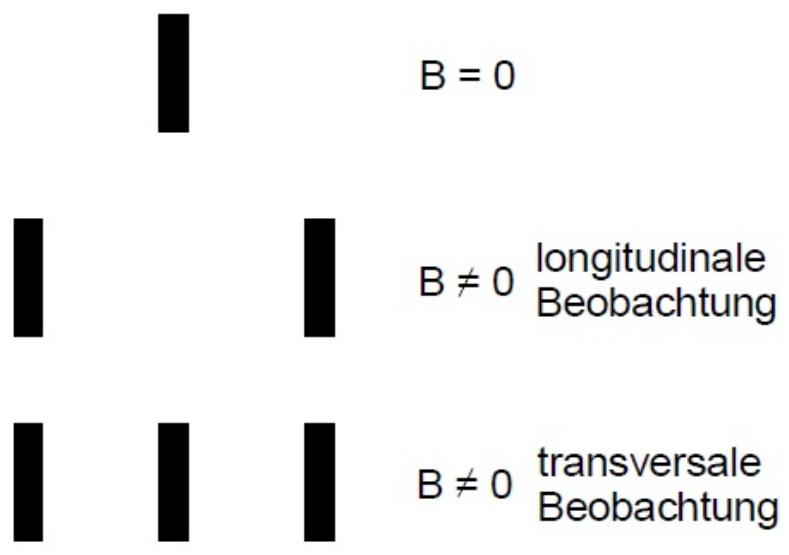
\includegraphics[scale=0.2]{polarisation.png}
    \vspace{-10pt}
    \vspace{3pt}
    \caption{Aufspaltungsbilder abhängig vom Beobachtungswinkel \cite{V27}.}
    \label{fig:pol}
\end{figure}

\noindent
Um eine Aufspaltung des Lichts in seine Spektren zu bekommen ist wie oben schon erwähnt ein Prisma in den Versuchsaufbau inkludiert. Dadurch werden im wesentlichen 3 Spektrallinien
sichtbar, rot, blau und grün. Die grüne Spektrallinie wird nur genutzt um den Aufbau zu justieren. Anhand der roten Linie wird der normale Zeeman Effekt untersucht und anhand der 
blauen der anormale.  


\noindent
Die Lummer-Gehrcke-Platte wird genutzt um ein Interferenzmuster zu erzeugen um mithilfe dessen die Wellenlängenverschiebung der Spektralinien durch das B-Feld berechnen zu können.
Dafür wird mithilfe eines Prismas der Lichtstrahl in eine Glasplatte mit planparallelen Flächen gelenkt. An jeder Grenzfläche der Plaspallte wird das Licht reflektiert, jedoch nicht
vollständig, sodass ein Teil dessen die Glasplatte verlässt. Die schematische Darstellung ist in \autoref{fig:Lum} dargestellt.

\begin{figure}[H]
  \centering
  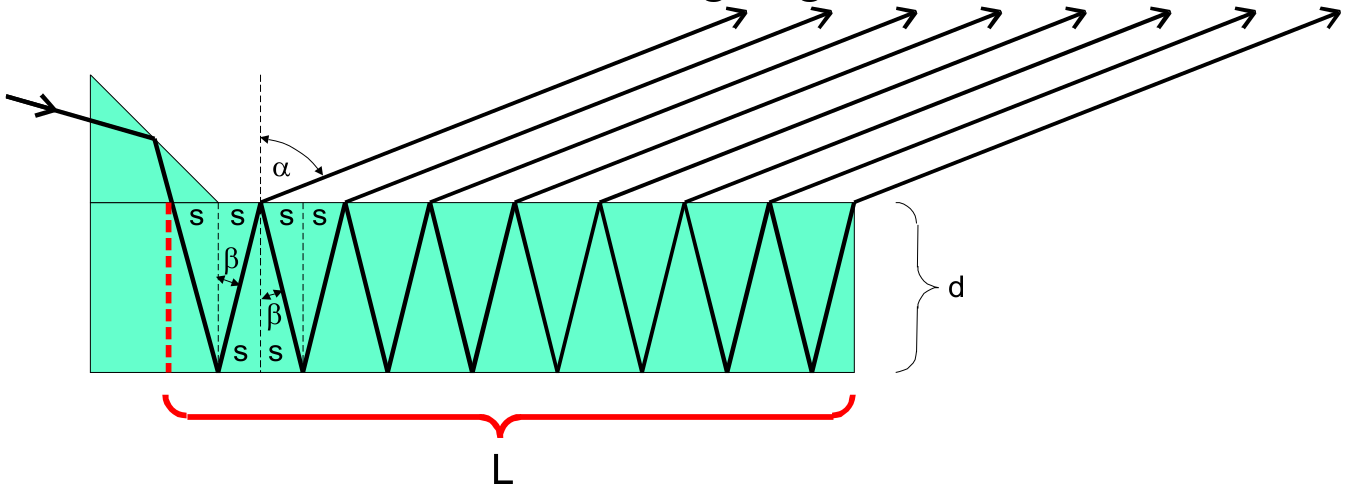
\includegraphics[height=6cm]{Lummer.png}
  \caption{Funktionsweise einer Lummer-Gehrcke-Platte \cite{V27}}
  \label{fig:Lum}
\end{figure}

\noindent
Das Interferenzmuster entsteht aufgrund konstruktiver Interferenz der austretenden Lichtstrahlen. Diese ist zu beobachten, wenn die Bragg-Bedingung 

\vspace{-5pt}
\begin{equation}
    2 \cdot d \cdot \text{cos}(\beta) = n \cdot \lambda \: , 
    \qquad n = \frac{\text{sin}(\alpha)}{\text{sin}(\beta)}
\end{equation}

\noindent
 erfüllt ist. $n$ gibt dabei den Brechungsindex an.

\noindent
Durch das Magnetfeld findet eine Verschiebung der Wellenlängen statt, sodass die Interferenzmaxima um den Faktor $\partial s$ verschoben werden.

\noindent
Die maximal Differenz, die zwischen den Wellenlängen zweier Strahlen bestehen darf, ohne dass diese sich überlagern, ist definiert als Dispersionsgebiet


\begin{equation}
    \Delta \lambda_\text{D} = \frac{\lambda^2}{2d} \sqrt{\frac{1}{n^2-1}}\, .
    \label{eqn:lam}
\end{equation}

\noindent
Das Auflösungsvermögen der Platte kann berechnet werden durch 

\vspace{-5pt}
\begin{equation}
    A = \frac{\lambda}{\Delta \lambda_\text{D}} = \frac{L}{\lambda} (n^2 -1) \, ,
    \label{eqn:a}
\end{equation}

\noindent
wobei dieses den minimalen Abstand zweier Beobachtungsobjekte angibt, welche klar von einander getrennt aufgelöst werden können. Relevant ist dies, da entfernte Punkte nicht als Punkte,
sondern als Beugungsscheiben, sogenannte Airy-Scheibchen, mit dem Radius $ R = 1,22 \lambda \frac{f}{D}$ durch die Platte dargestellt werden. Dabei gibt $D$ den Durchmesser der 
Linse an. 

\noindent
Damit 2 Objekte getrennt von einander aufgelöst werden können muss das Helligkeitsmaximum der einen Airy-Scheibchen auf dem ersten Helligkeitsminimum des anderen Airy-Scheibchen liegen.
\footfullcite{Spektrum}

%\begin{thebibliography}{1}
%  \bibitem{spektrum} \textit{Auflösungsvermögen}, Spektrum.de, Online, 2022-07-08.
%\end{thebibliography}

\subsection{Messung}
Für die Aufnahme der Messwerte muss zuerst die Stärke des Magnetfelds bestimmt werden. Dafür wird mittels einer Hallsonde die ins Magnetfeld geschoben wird, die Stärke dessen In
$0,5$A Schritten von 0A bis 5A durchgemessen. 

\noindent
Danach wird der Aufbau justiert und mittels der Platte mit dem Spalt durch verschieben einmal die rote und einmal die blaue Spektrallinie ausgewählt, da diese durch das Prisma 
räumlich getrennt wurden. 

\noindent
Es werden jeweils für die rote und die blaue Spektrallinie 2 Fotos mit eingeschaltetem Magnetfeld und 2 ohne eingeschaltetem Magnetfeld aufgenommen. Nach jedem Foto wird der Polarisationsfilter
um 90° verdreht.

